\documentclass{beamer}
\usetheme{metropolis}

% my Colors
\definecolor{HS-Blue}{HTML}{185363}

% Change the primary color
\setbeamercolor{palette primary}{bg=blue, fg=white}
\setbeamercolor{frametitle}{bg=HS-Blue}

% Optional: Customize other colors
\setbeamercolor{title separator}{fg=HS-Blue}
\setbeamercolor{progress bar}{fg=HS-Blue}
\setbeamercolor{block title}{bg=blue!70, fg=white}
\setbeamercolor{block body}{bg=blue!20, fg=black}

\title{Erkennung von Kerben in medizinischen Stents mit Hilfe von neuronalen Netzwerken}
\subtitle{\small Notch detection on medical stents using neural networks}
\author{Yves Seburger}
\date{10.07.2024, 19.07.2024 oder 26.07.2024}
\institute{Hochschule Kaiserslautern\newline
Schoenstr. 11\newline
67659 Kaiserslautern}
\setbeamertemplate{frametitle}
{
    \begin{beamercolorbox}[wd=\paperwidth,ht=3ex,dp=1.125ex,leftskip=0.3cm,rightskip=0.3cm]{frametitle}
        \insertframetitle
        \hfill
        \raisebox{-0.19cm}{
\includegraphics[height=0.74cm]{Bilder/HSKLLogo - white font.png}}
         
    \end{beamercolorbox}
}

\begin{document}

\frame{\titlepage}

\begin{frame}
\frametitle{Überblick}
\tableofcontents
\end{frame}

\section{Aufgabenstellung}
\begin{frame}[allowframebreaks]
\frametitle{Aufgabenstellung}
\begin{itemize}
    \item Aufnahme von Stentbildern \newline
        \begin{figure}
            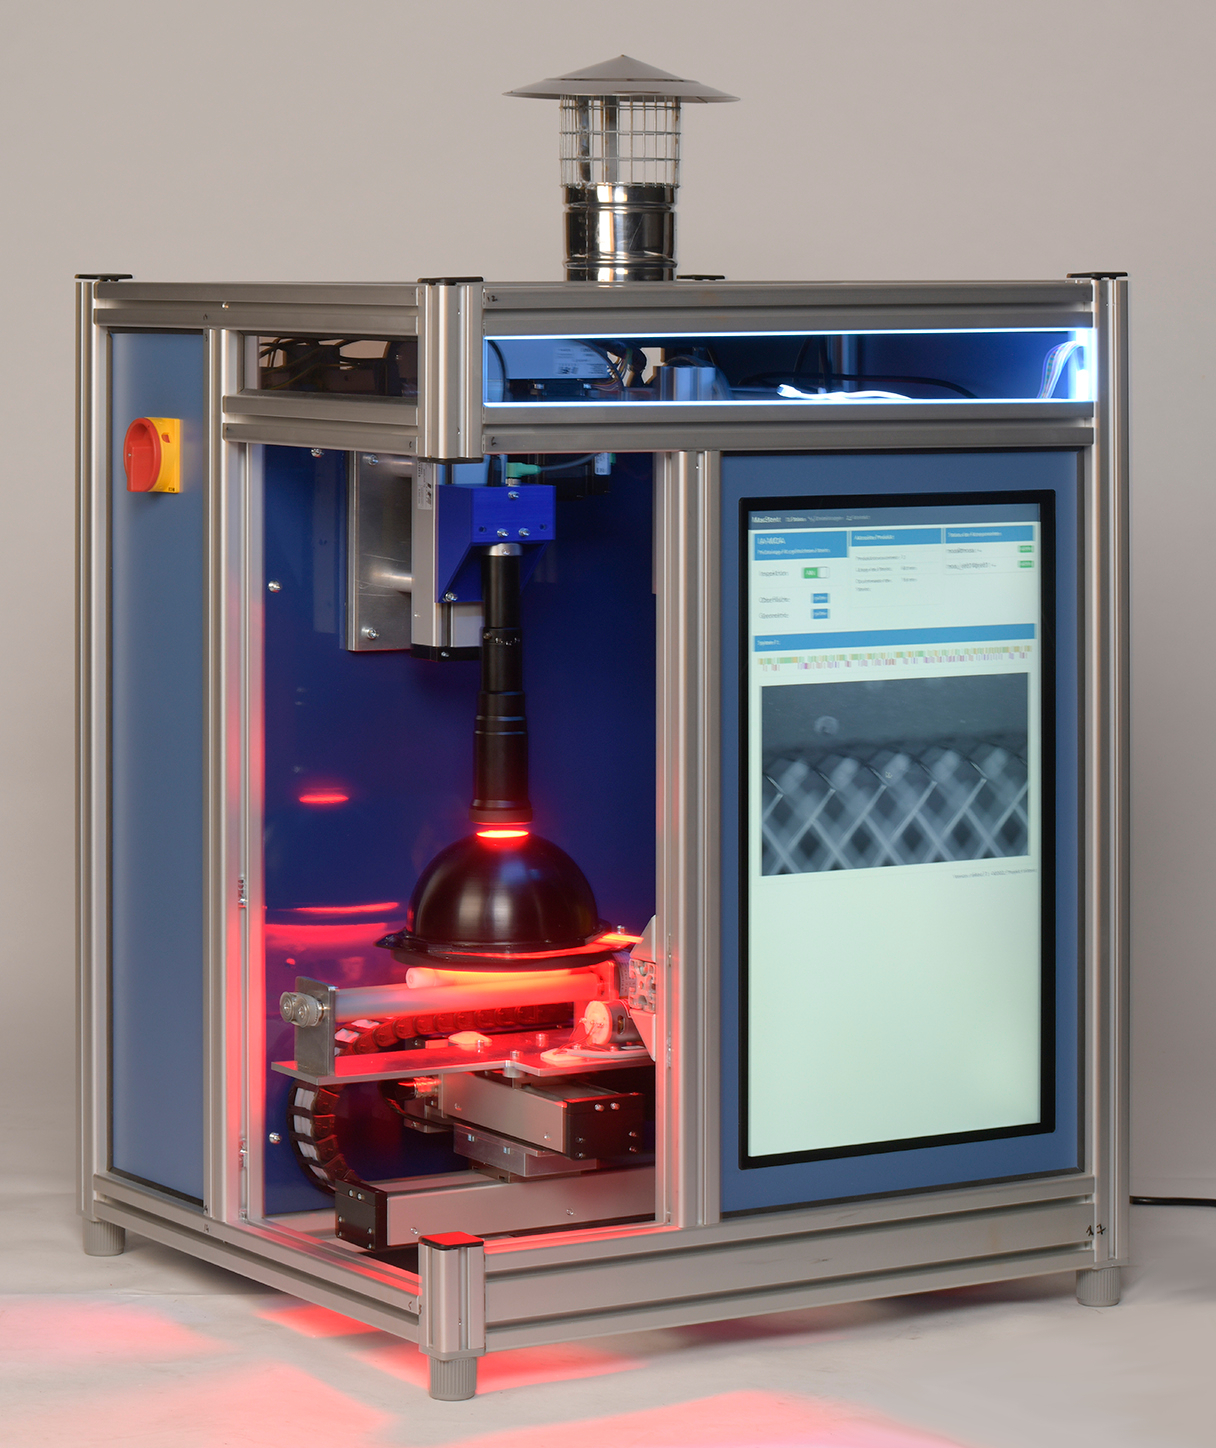
\includegraphics[height=4.5cm]{Bilder/MoA_Gesa_preversion_cut.jpg}
            \hspace{20px}
            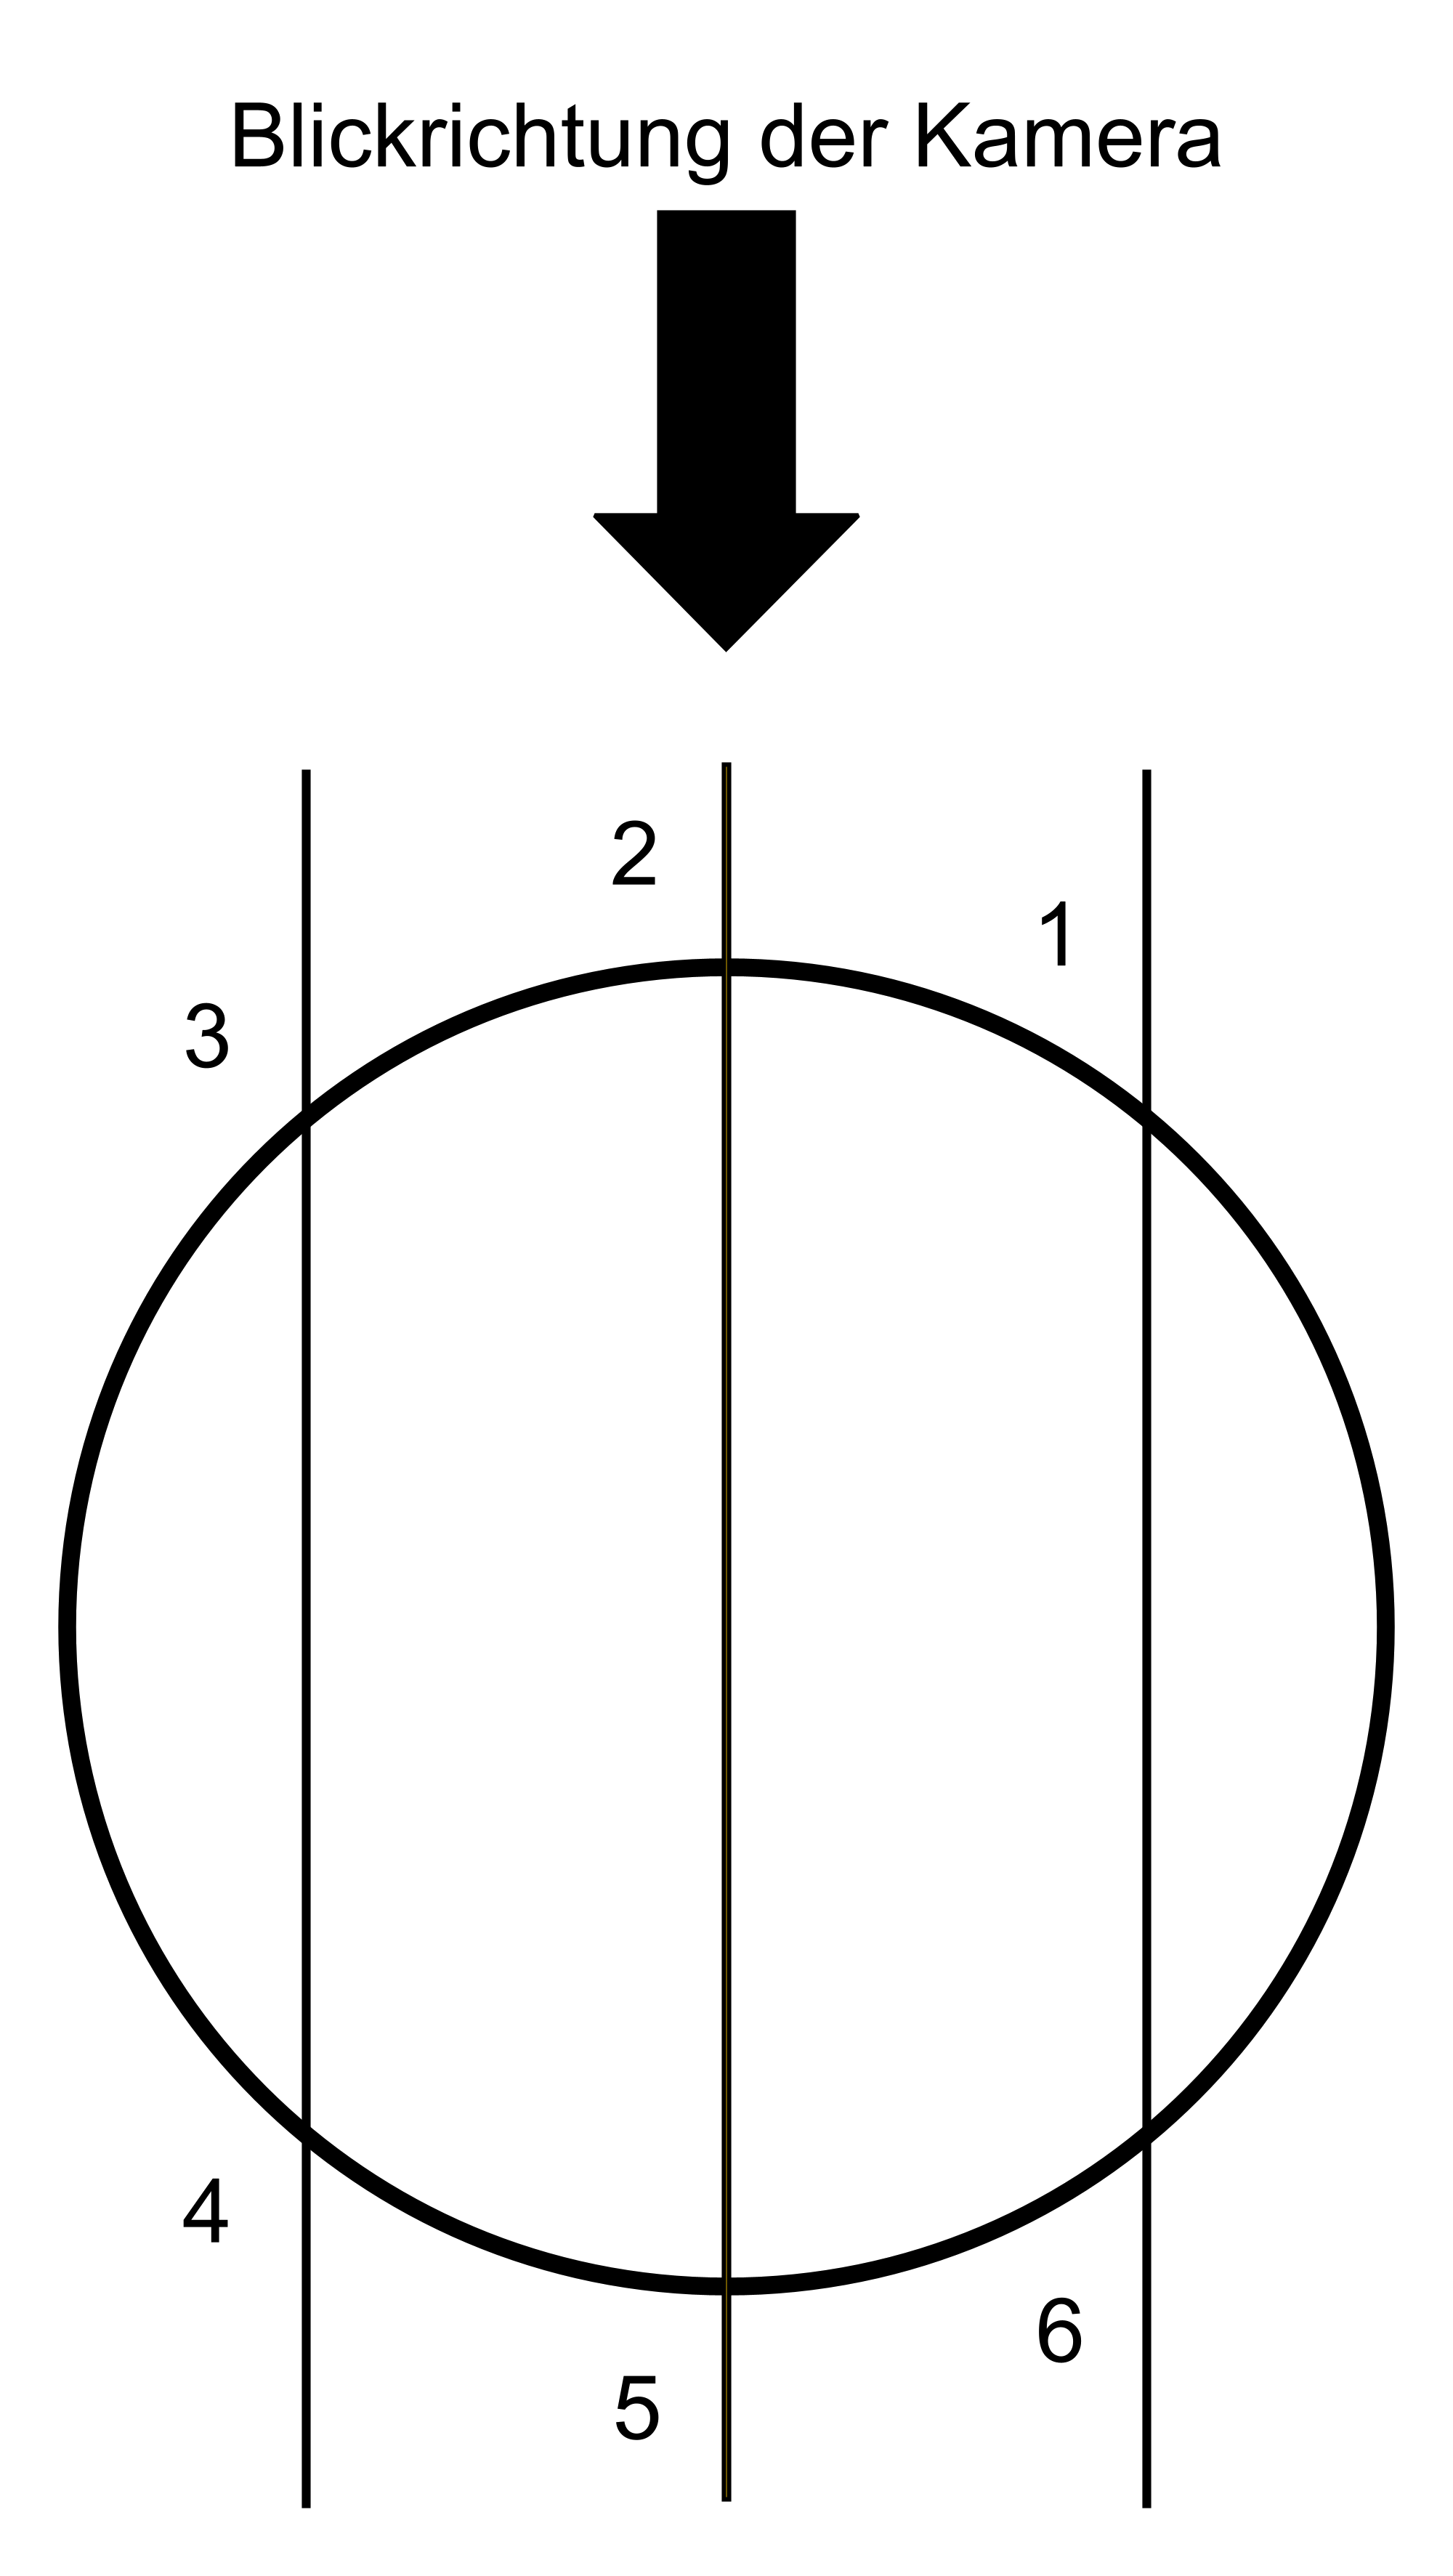
\includegraphics[height=4.5cm]{Bilder/Stentpositionen.png}
            \caption{((links) MoA Quelle: Dipl.-Ing Viktor Truderung, (rechts) Stentpositionen. Quelle: Yves Seburger)}
        \end{figure}
        \begin{figure}
            \includegraphics[width=10cm]{Bilder/Stent.jpg}
            \caption{(Aufnahme eines Stentteils. Quelle: Yves Seburger)}
        \end{figure}  
\end{itemize}
\begin{itemize}
    \item Einschränkung von Kerbenfehlern \newline
        \begin{figure}
            
\includegraphics[width=4cm]{Bilder/Annotationfragen/Frage_5_crop.jpg}
            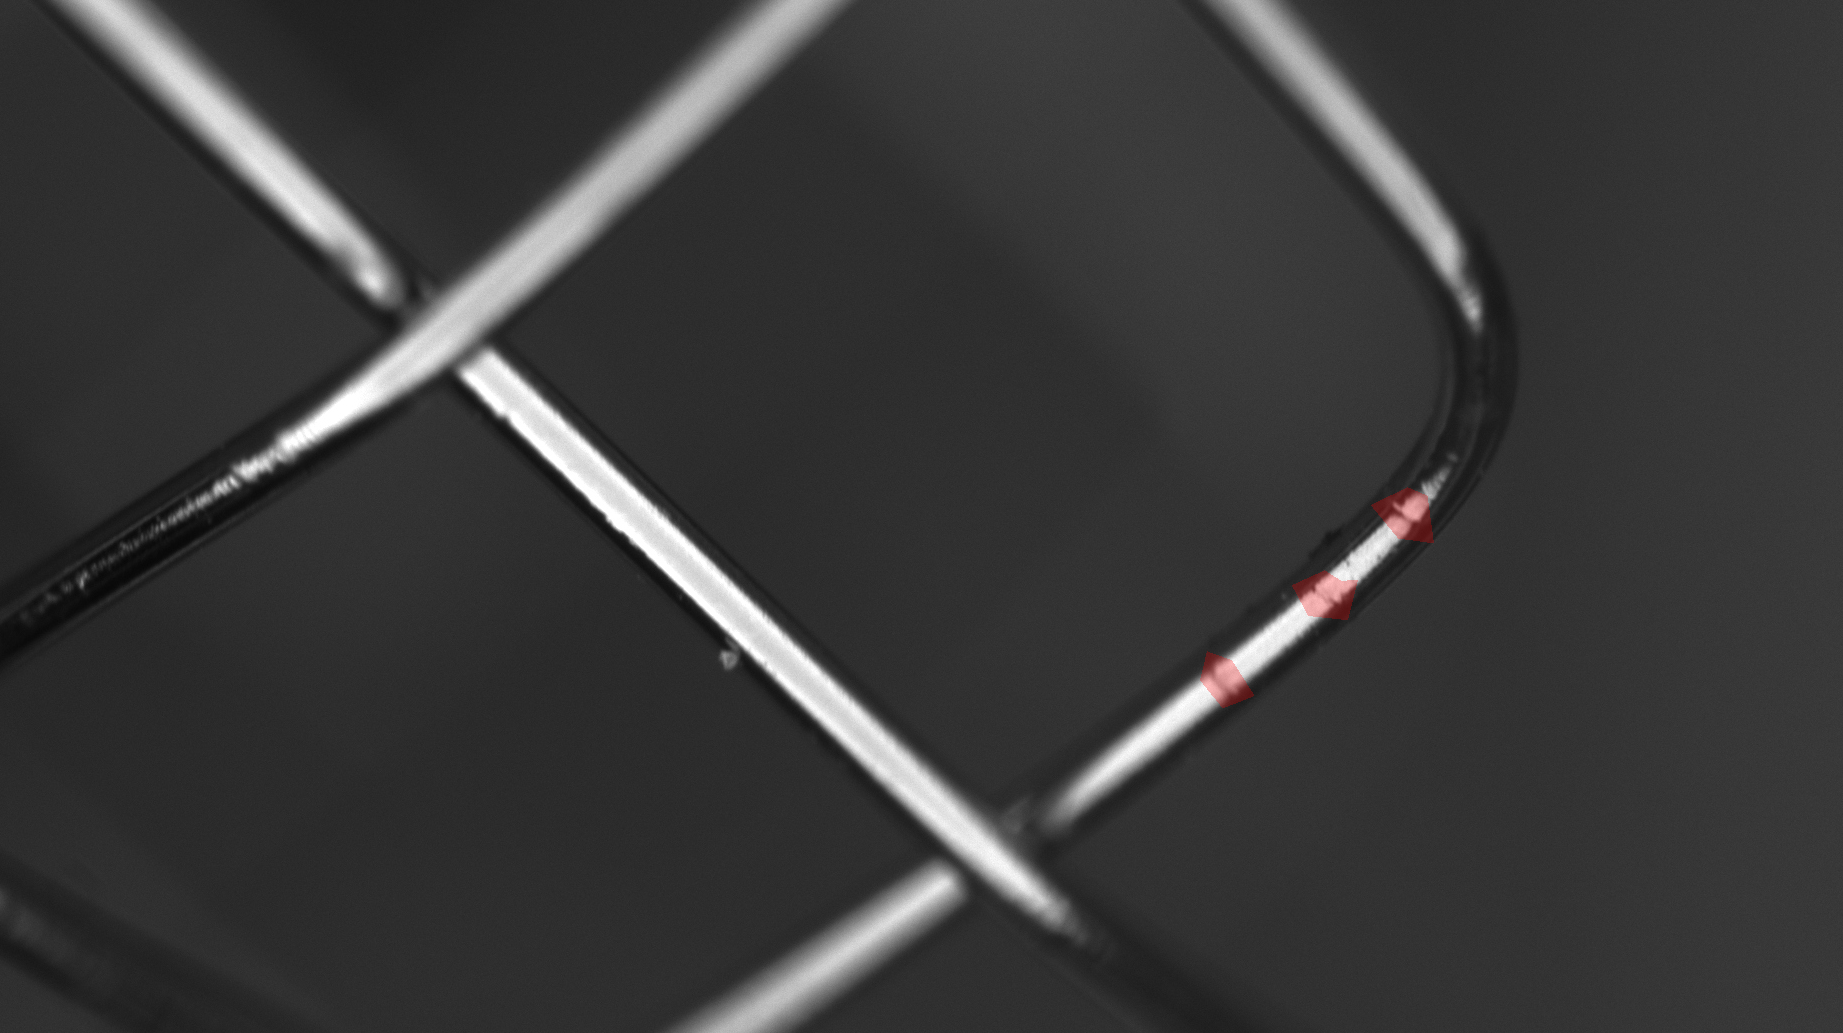
\includegraphics[width=4cm]{Bilder/Annotationfragen/Frage_5_anno.png}
            
\includegraphics[width=4cm]{Bilder/Annotationfragen/Kratzer.jpg}
            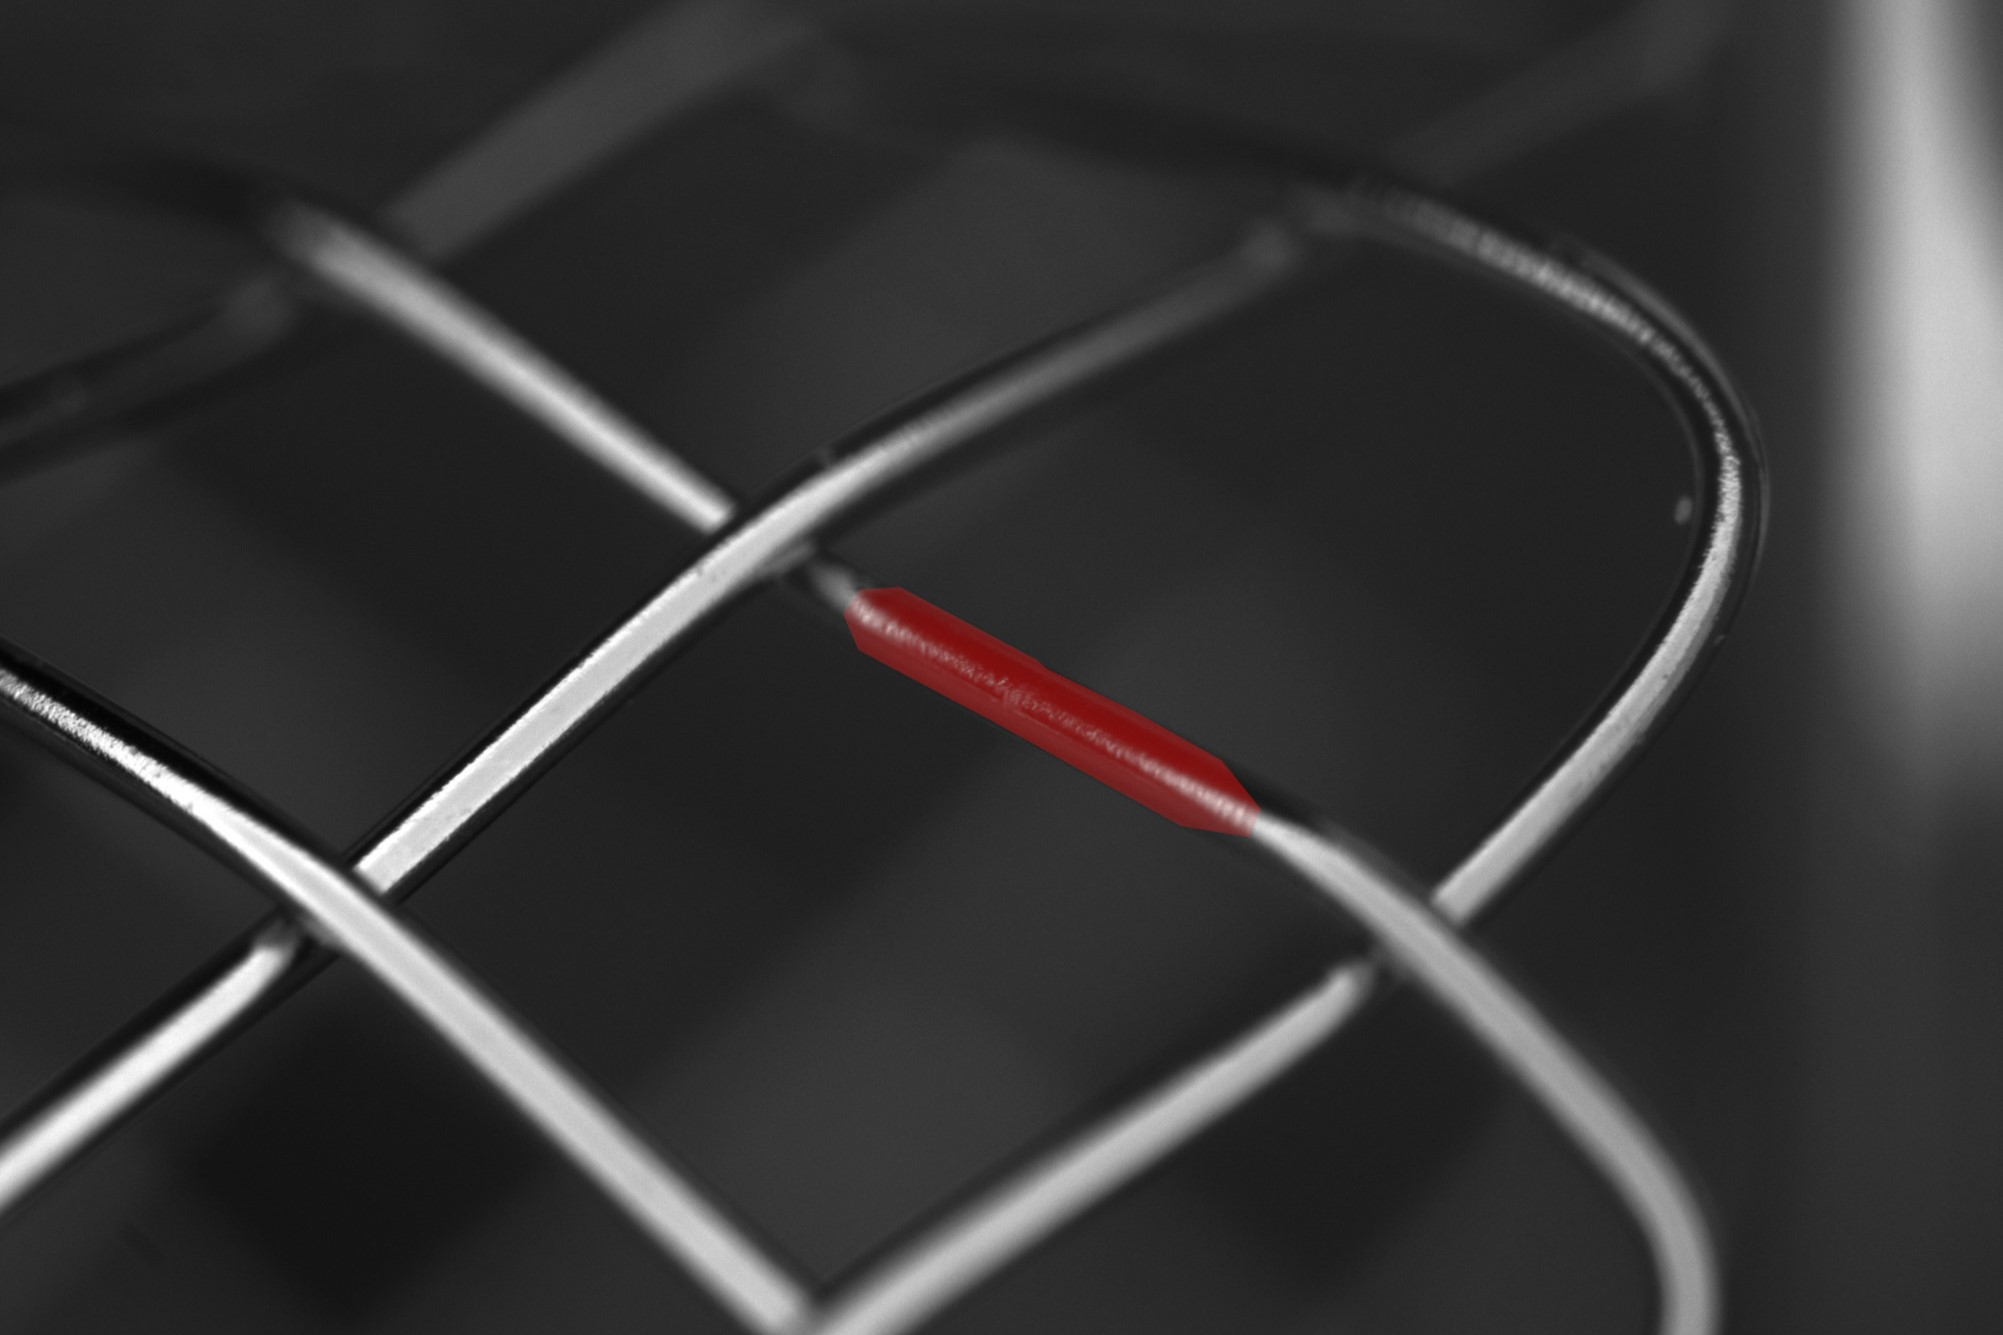
\includegraphics[width=4cm]{Bilder/Annotationfragen/Kratzer_anno.jpg}
            \caption{Annotierte Bilder. Quelle: Yves Seburger}
        \end{figure} 
    \item Annotation \newline
    \begin{figure}
        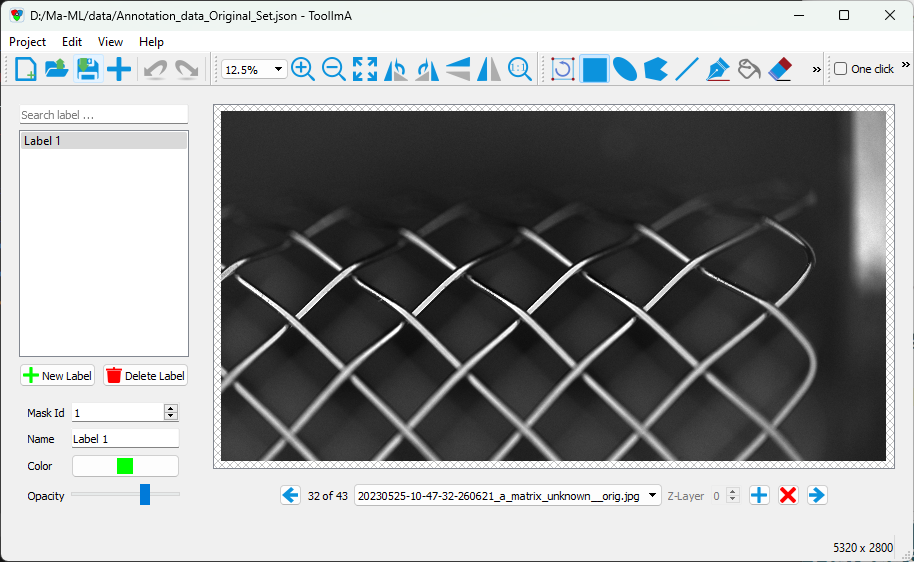
\includegraphics[width=8cm]{Bilder/toolima.png}
        \caption{Toolima, Software zu Annotation. Quelle: Yves Seburger}
    \end{figure} 
    \item Programmerstellung
        \begin{itemize}
            \item Inspiration (Aladdin Persson, Thomas Zimmermann)
            \item 
        \end{itemize}
    \item Training
    \item Validierung
\end{itemize}
\end{frame}

\section{Probleme}
\begin{frame}
\frametitle{Probleme}
\begin{itemize}
    \item normaler Dice-Score
    \item Anzahl der Originalbilder
    \item Fehlerannotierung
    \item Aufteilung der Originaldaten
\end{itemize}
\end{frame}

\section{Methodik}
\begin{frame}
\frametitle{Methodik}
\begin{itemize}
    \item gewichteter Dice-Score
    \item Augmentierung
    \item UNET und Half-UNET
    \item Auswahl des Datasets
\end{itemize}
\end{frame}

\section{Resultate}
\begin{frame}
\frametitle{Resultate}
\begin{itemize}
    \item verschiedene Trainingssets
    \item Dice-Score vs. gewichteter Dice-Score
    \item UNET vs. HalfUNET
    \item versch. Lernraten im Test
    \item versch. Bildauflösungen
    \item Endresultate
\end{itemize}
\end{frame}

\section{Fazit und Ausblick}
\begin{frame}
\frametitle{Fazit und Ausblick}
\begin{itemize}
    \item Erweiterung der Aufnahmen
    \item Tests mit veränderlichem $\alpha$
    \item Nutzung anderer Trainingssets (Autos, Vögel, etc.)
\end{itemize}
\end{frame}

\end{document}
